\section{Plano e Método de Trabalho}
\label{sec:chap01_workmethodology}
Um plano de trabalho é uma ferramenta importante na gestão de qualquer projeto, na medida em que permite ter visibilidade da sua extensão temporal, das tarefas a realizar e do período associado a cada uma delas. Na Figura~\ref{fig:planning-gantt_chart} demonstra-se o diagrama de \textit{Gantt}, contendo as tarefas inerentes a cada uma das fases do projeto, descriminadas na tabela abaixo.

\begin{table}[!ht]
\caption{Fases do projeto, periodicidade e respetiva duração}
\label{tab:project-phases}
\centering
\resizebox{\textwidth}{!}{\begin{tabular}{l|l|l|l}
%
\toprule
%
\tabhead{Fase do Projeto}&\tabhead{Data Prevista de Início}&\tabhead{Data Prevista de Fim}&\tabhead{Duração (dias)}\\ 
%
\midrule
Conceção                 & 01-Jan-2019                      & 16-Fev-2019                   & 46                      \\
Análise                  & 11-Fev-2019                      & 08-Março 2019                 & 25                      \\
Desenvolvimento          & 04-Março-2019                    & 17-Maio-2019                  & 74                      \\
Validação                & 17-Maio-2019                     & 12-Junho-2019                 & 26                      \\
Documentação             & 01-Jan-2019                      & 30-Junho-2019                 & 180                     \\ 
%
\bottomrule
\end{tabular}}
\end{table}

A Tabela~\ref{tab:project-phases} carece de informação sucinta de cada uma das fases, pelo que se passam a descrever:

\begin{itemize}
    \item
    {
        \textit{Conceção} -- engloba as tarefas que relacionadas com o problema, o seu enquadramento, o estudo do valor e estado da arte. Ou seja, a visão do projeto;
    }
    \item
    {
        \textit{Análise} -- nesta fase, faz-se o levantamento dos requisitos, a escolha e definição da semântica de domínio, estipulam-se a(s) tecnologia(s) a utilizar e especifica-se a arquitetura para o módulo. A presente fase consiste no estudo e preparação para o desenho da solução; 
    }
    \item
    {
        \textit{Desenvolvimento} -- desenvolve-se a solução conjeturada na fase anterior, envolvendo um período de experimentação de código base da arquitetura definida (para possível reestruturação ou ajuste);
    }
    \item
    {
        \textit{Validação} -- avalia-se a solução com base nos critérios definidos na secção~\ref{sec:chap01_solutionevaluation} e consequentemente, podem-se registar melhorias para o módulo. É nesta fase que também se demonstra a solução às partes interessadas do trabalho (\exempligratia{\gls{ceo}, \gls{cto}, {\supname}, orientador do projeto, {\cosupname}, responsável pelo projeto etc.});
    }
    \item
    {
        \textit{Documentação} -- engloba a escrita da tese como veículo de transmissão de conhecimento obtido e de outros documentos de suporte, a serem usados no contexto empresarial (\exempligratia{documento de especificação de requisitos de \textit{software}, especificação arquitetural de \textit{software}, manual de instalação e outros que façam sentido}).
    }
\end{itemize}

Quanto ao método de trabalho a seguir na realização deste trabalho, são considerados os seguintes passos:

\begin{enumerate}
    \item 
    {
        \textit{Revisão de literatura disponível sobre o contexto do problema} -- com o objetivo de perceber o estado atual do {\productname} e as implicações que o módulo trará, assim como concluir acerca do valor da solução para o produto;
    }
    \item
    {
        \textit{Revisão de literatura existente acerca de \gls{pln} e paradigmas arquiteturais relacionados} -- adquirir conhecimentos sobre técnicas e ferramentas de \gls{pln}, principalmente analisando soluções já existentes, identificando aspetos relevantes para o trabalho e outros que não foram contemplados;
    }
    \item
    {
        \textit{Idealização do módulo} -- depois da análise dos conhecimentos adquiridos com as revisões realizadas nos passos descritos anteriormente, parte-se para o levantamento dos requisitos junto das partes interessadas do projeto, resultando na concepção de um módulo capaz de lhes dar resposta; 
    }
    \item
    {
        \textit{Estudo do domínio de negócio} -- com o intuito de entender a semântica do negócio em questão e definir um dicionário a ser usado pela solução;
    }
    \item
    {
        \textit{Implementação do módulo e validação} -- o foco é pôr em prática a solução conceptualizada nas fases anteriores. Após a implementação, são realizam-se testes com vista a perceber se os resultados obtidos são os esperados e proceder às melhorias que forem evidentes;
    }
    \item
    {
        \textit{Elaboração da documentação} --  por fim, passa-se à escrita do presente documento e de documentos de suporte, baseando-se nas observações, nas experiências e conclusões obtidas ao longo do projeto.
    }
\end{enumerate}

\clearpage
\begin{sidewaysfigure}[!ht]
    \centering
    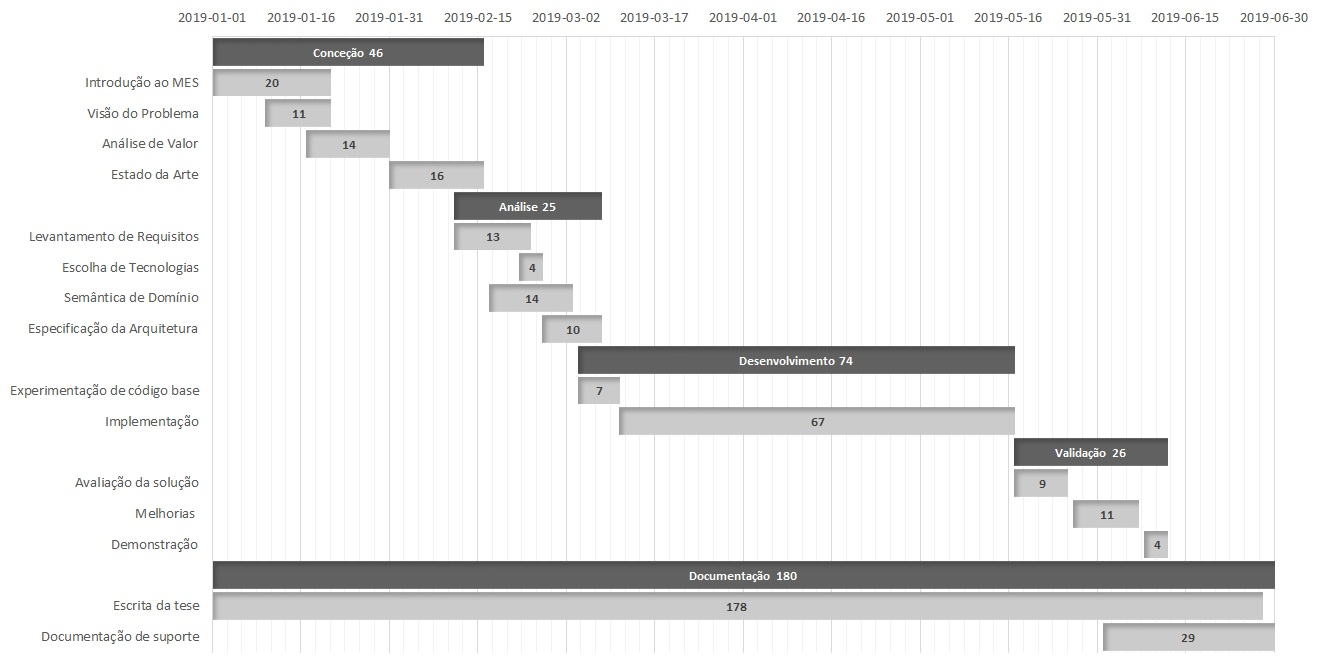
\includegraphics[width=1.0\textwidth]{ch01/assets/gantt.jpg}
    \caption{Diagrama de \textit{Gantt} referente ao planeamento do projeto}
    \label{fig:planning-gantt_chart}
\end{sidewaysfigure}
\clearpage